\subsection{Quantitative data}

    %What the data said

    % Christine och Patrick berättade senare att i regel presterar Young Mentor lite bättre än CBT, enligt deras rakningar. (från iteratoin 1 - stämde detta?)

    % Relevans av att testa financial literacy: "Precis som med förra gruppen, verkar ekonomin vara det svåraste att förstå (dolda utgifter, hur gå med vinst), som youth." (från iteration 1)

% Important to be objective
% En diskussion om hur resultaten kan användas i praktiken är också i de flesta fall belysande och relevant i rapporter

% https://liu.se/ias/kontakta-oss?l=en

For the first time, automatic data collection was used, which increased the amount of quantitative data that could be analysed substantially. Below, the findings from each data analysis method are presented.

\subsubsection{Google Sheets} \todo{Add table from Google Sheets}
For results from the Google Sheets, see figure \ref{analys4spreadsheet}. Early observations from the pre-test data when inserted into Google Sheets was that a surprising number of cells were left blank. One user had not done the pre-test, where some had left questions unanswered (most commonly "Do you own a company?" (should have used the word "business"), plus "Hours of preperation" and "Occations for a youth session" (there is a tendency this might be because they were not proud of their answers, because of correlations with low quiz results).

\begin{figure}[h]
    \centering
    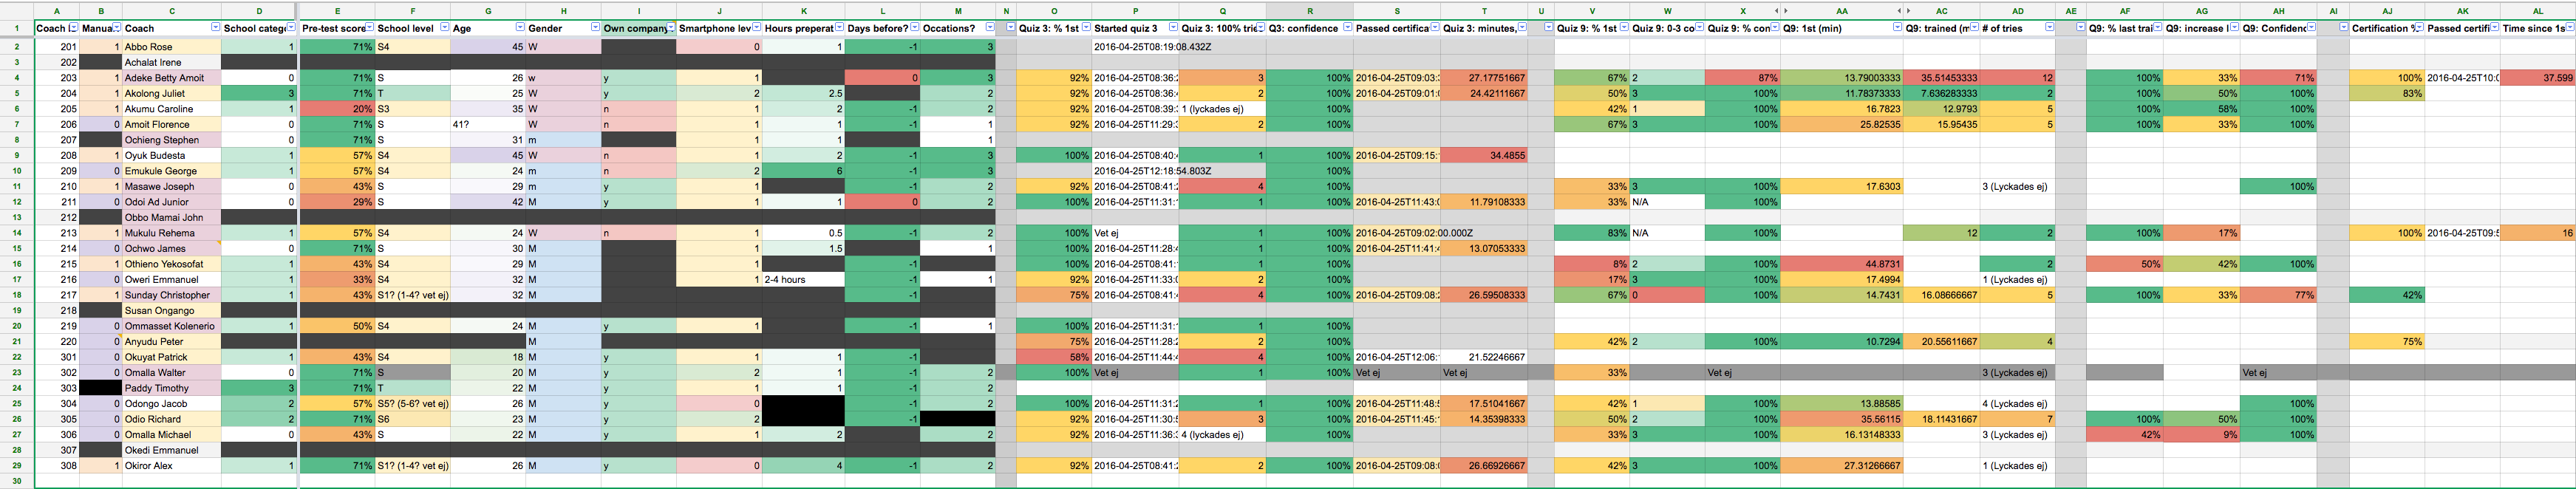
\includegraphics[width=1.0\textwidth]{analysis/analys4spreadsheet.png}
    \caption{The Google Sheet after merging the pre-test data and the summed quiz results data.}
    \label{fig:analys4spreadsheet}
\end{figure}

Missing cells was not as obvious with the app results, were users could not progress in a quiz without answering both the question and the confidence. However, none of the passed quiz 9 certification answers had been submitted. Thus, it was needed to add these from the manual recordings, which had been used as a backup in case anything like this would happen.

There were a number of quick insights that could be drawn before the parallell coordinates visualization, simply by looking at the data as a spreadsheet.

It was believed that smartphone users feeling like novices might have a disadvantage with the app, since they will not learn as fast as experienced users. The interactions shows however, between iteration 3 to 4, almost all of the coaches does not feel intermediate instead of beginners using the smartphone and the YoungDrive app. The quiz data verifies this, with no direct correlation between technical skills and quiz results. From the pre-test data, it can be seen that only CBTs said they didn't feel comfortable with smartphone (n=2, of which there were 6 Youth Mentors and 14 CBTs). A reason might be age, as CBTs were older than the Youth Mentors. Also, youth mentors had higher school level than the CBTs. More probable, is that the experience of using a smartphone since iteration 3 has matured over time, and that they are now more confident. %It is interesting that this has improved since iteration 3, possibly indicating that the smartphone skills have matured since the last test two weeks ago.

From the Google Sheets quiz results data, it could be seen that there was a surprisingly low number of answers where the user answered the question without confidence.  This is not good for feedback purposes, as answers were actually often not correct.

Also, more users had started a quiz without finishing it than anticipated. This speaks for usability issues (cancelling the quiz by mistake, like cklicking the back button, or loss of internet access) or bad technical skills (needs to design to be more fail-safe) or lack of motivation (needs to design for unmotivated coaches as well. The need group of "challenged coaches" might need other design than "ideal coaches".

Finally, a lot of users had done quizzes that were not Topic quiz 3 and Coach quiz 9, which might indicate high interest (if they did more than 2 quizes) or confusion (if they did not do 3 or 9, but they did do other quizes) during the app evaluation. This meant that on some aspects, there were less data than anticipated, (which was troublesome, as there were already few data points), and some aspects where there was more data than anticipated (on overlooked other quizzes).

First-hand insights before the parallell coordinates were that there was a strong corrolation between pre-quiz results and quiz 9 try 1 (slightly visible also in quiz 3 try 1, but with more outliers). Also, with manuals there was a higher probability to finishing quiz 9 training and certification (see also findings from the parallell coordinates visualization below). The data shows small tendencies that being honest and deliberate during the training increases the likelihood that a coach can get 100\% without faults, and has truly learned.

The final version of the app shows users can get 100\% on quiz results much faster that the previous version, where the score board had been improved. Since the target group in Zambia and Uganda was different, it is hard to empirically prove if it went faster getting 100\% with the possibility of repeating only the wrong questions, asking "Are you sure?", and providing individual feedback. Asking after the app does in iteration 4 does show however, that 100\% of the coaches now thought the feedback was good for learning.

\subsubsection{Statistical analysis}
Statistical analysis in R unfortunately showed that none of the results were statistically significant to be notable using linear regression, or any of the other statistical methods detailed in the methodical framework. It was believed that statistical analysis could at least give insight into what to look after in the parallell coordinates visualization, but also for this, a larger samle would be needed.

\subsubsection{Parallel coordinates visualization}
The interactive parallel coordinates visualization could give many more insights, more faster than the static presentations in Google Sheets.

There are an almost unlimited number of findings and observations that are interesting to look at via the parallel coordinates visualization. Even if there are no clear correlations (which are often found immediately when working with large data sets and parallell coordinates, see example from \ref{fig:terre}), tendencies can be found. As nothing is statistically significant (mostly because of the small data sample), the only thing that could be found are tendancies, and to analyze outliers. Then, these findings was critically analyzed to characteristics, and observations made from the app tests. As such, the data should be seen as indications of where future research is interested, and not as universal truths. For further research into the data, see figure \ref{fig:parallellCoordinates3} and the below sections.

\begin{figure}[h]
    \centering
    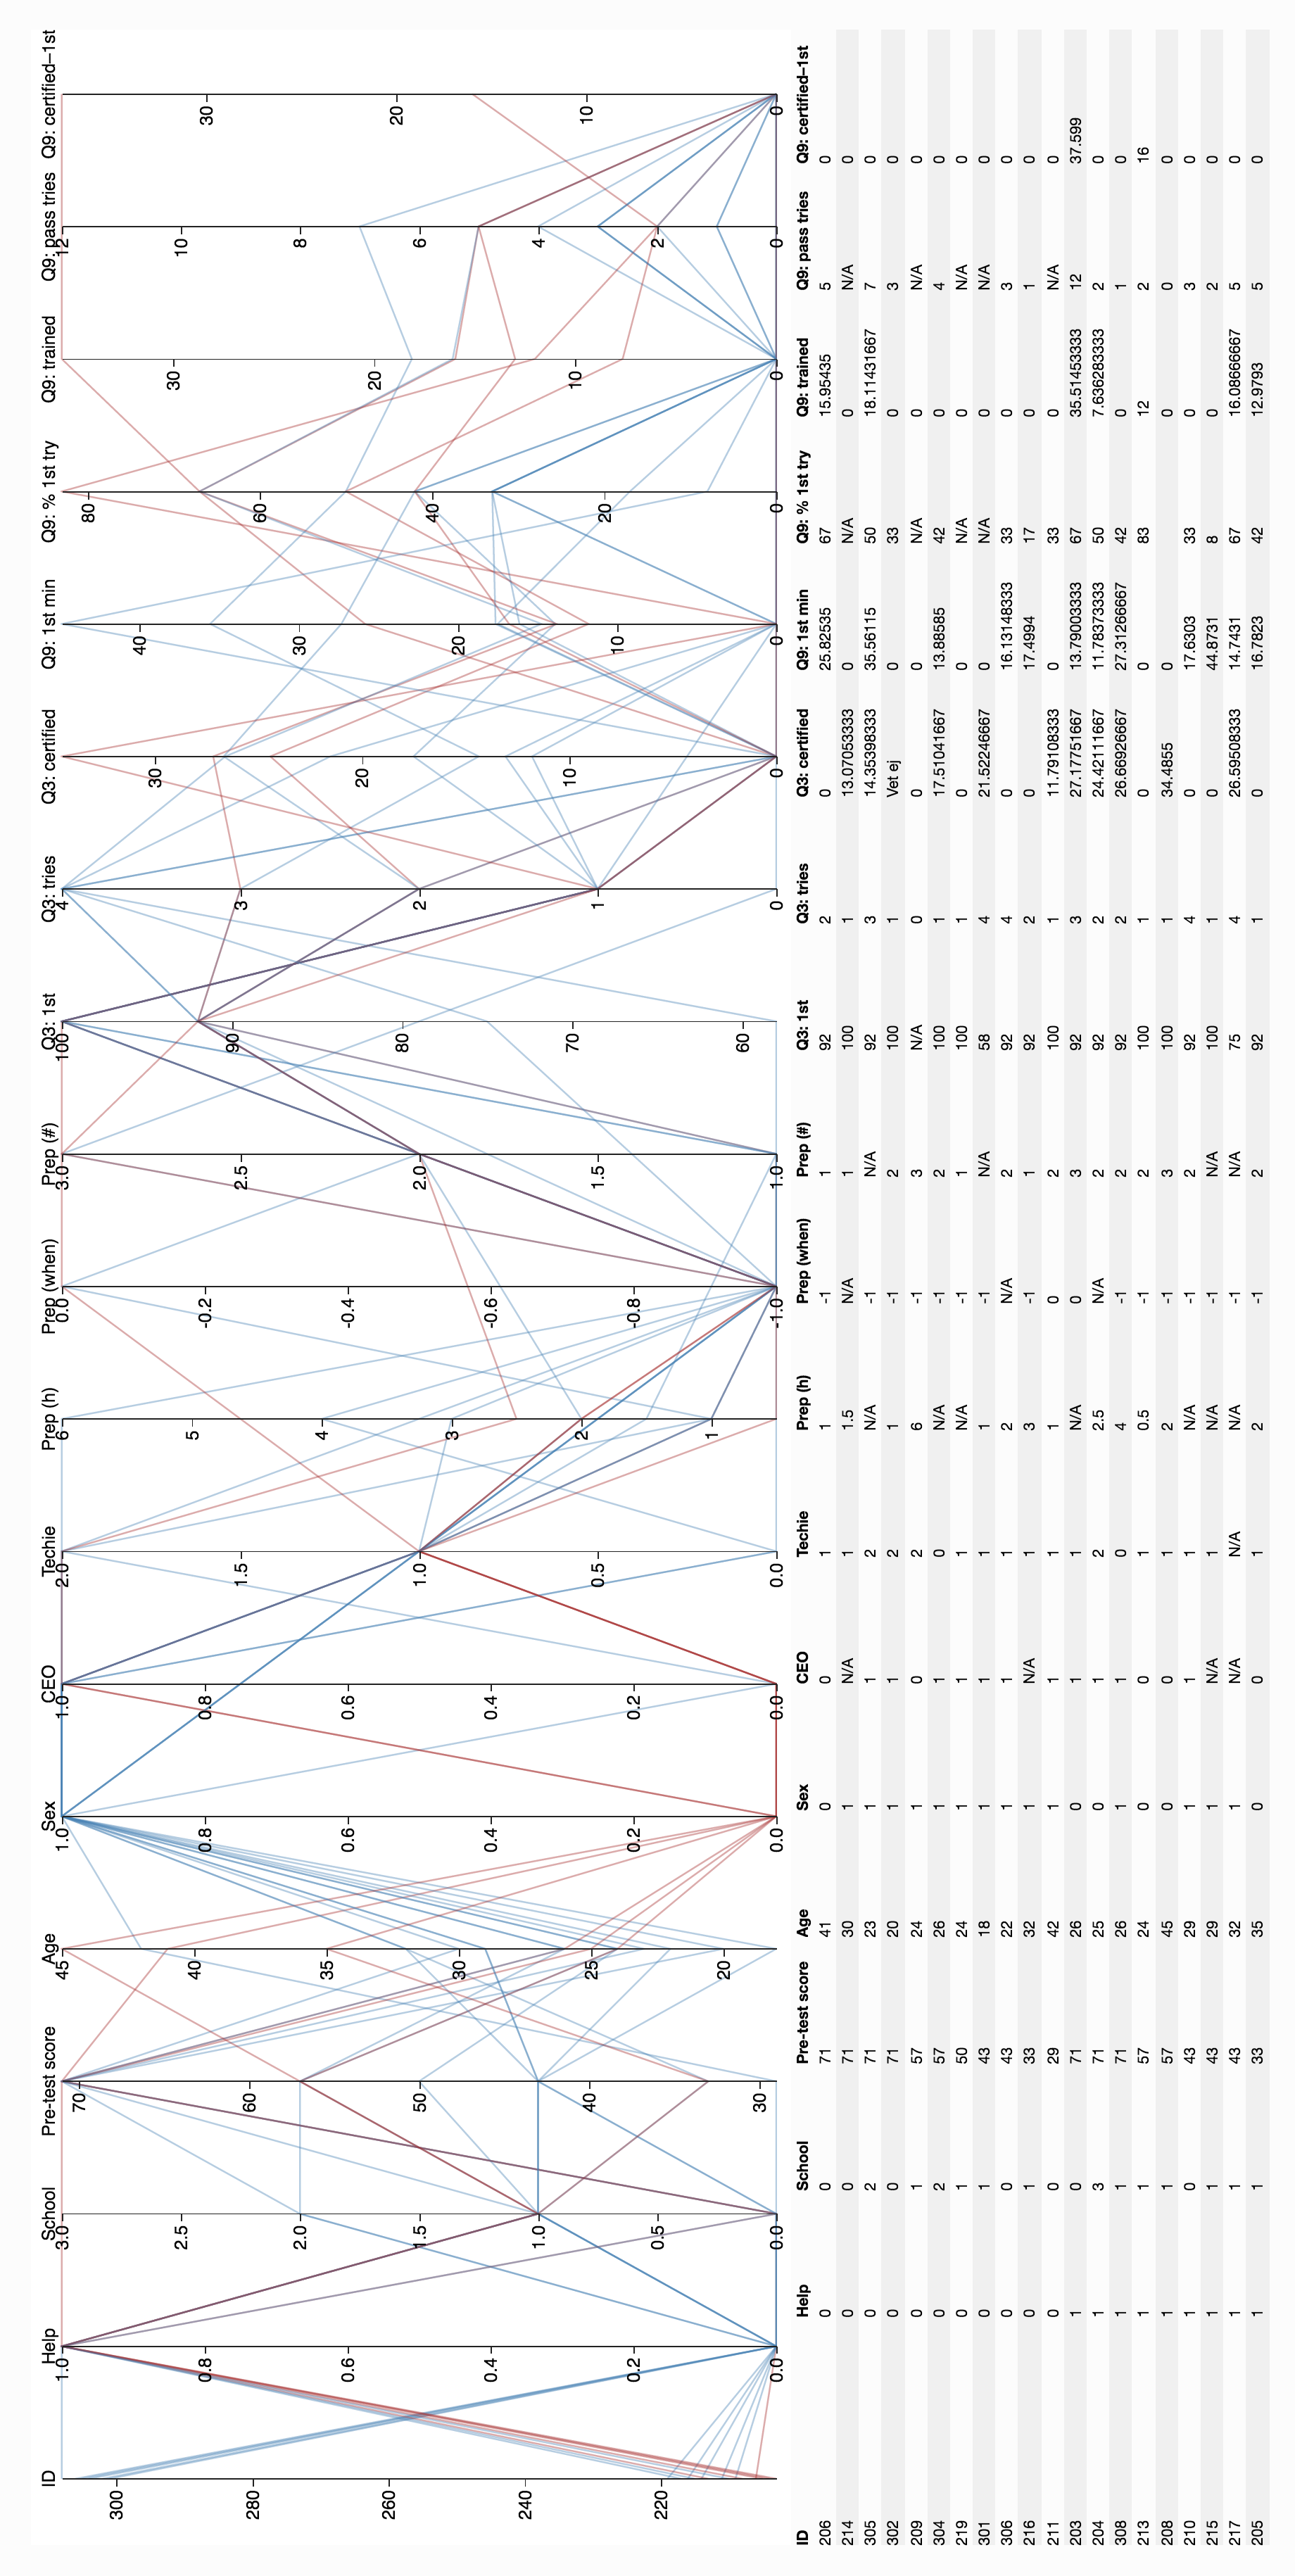
\includegraphics[width=1.0\textwidth]{analysis/parallellCoordinates3.png}
    \caption{The quiz results from iteration 4 shown in an interactive paralell coordinates visualization. The result is avaiable on \url{http://marcusnygren.github.io/youngdrive-parallel-coordinates/}.}
    \label{fig:parallellCoordinates3}
\end{figure}

\begin{figure}[h]
    \centering
    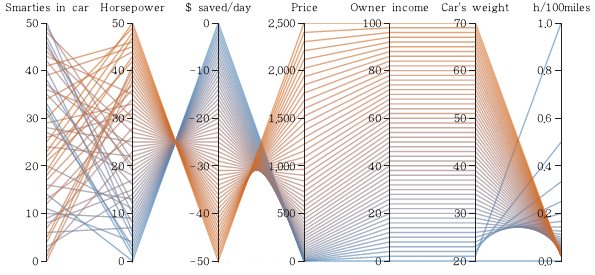
\includegraphics[width=1.0\textwidth]{analysis/terre.png}
    \caption{A parallel coordinates visualization example which shows clear correlations between different data points. Example from Lopez \cite{une-terre}.}
    \label{fig:terre}
\end{figure}

%* 1/6 Youth mentors had brought manual, compared with 8/14 CBTs
%* There are no female Youth Mentors (i.e. 100\% male Youth Mentors)
%* All of the YM's run their own businesses, compared with 5/10 for CBTs

%* Seemingly no difference CBT vs. YM in when prepares for session
%* All YM prepares 2 times for session, while CBT can train also 3 or 1 time)

%* 13/14 CBTs gjorde quiz 3 try 1, 6/6 YM's
In quiz 3 and 9, there is no unison difference in performance between Youth Mentors and CBTs. In quiz 9 however, the Youth Mentors are top performers compared to CBTs, which goes in line with the project leaders opinion in the field that Youth Mentors are slightly better in the field than the CBTs. It is important to note that there is nothing statistically significant to draw confident conclusions. Further research needs to be made, as a connection between how a coach performs in the field versus the app is valuable. %CBT 6/14 st certifierade, YM 4/6 st

%Quiz 9 (rött=CBT:
%* 6 CBTs gör ej Q9 try 1, 2 YM gör ej
%* YM är top performers på Q9 try 1 jämfört med CBTs
%* endast 1 YM klarade däremot träningen, medan
%* YM's är bättre på quiz 9 try 1 än CBTs
%* Det är endast 1/7 som klarade quiz 9 training som är Youth Mentor
%* Antal försök man gjorde är likvärdigt, förutom en YM som hade 12 försök (och klarade quiz)

%If the app is indeed an indicator if the coach performs well, the data shows that female coaches should be hired for YoungDrive.

The results shows that the ideal coach, according to the quiz app, would be a woman, since she has better knowledge in spite of having less formal education. She prepares more, is more aware of her own knowledge and has a better study technique, respecting the app feedback for meta-cognition and meta-memory.

It is very clear from the data that women have better quiz results and prepares more for their youth sessions, even though they have lower school education. More than average, for example in quiz 9, the women have a higher lowest treshold, and a much higher record, than the men. Only women (n=2) passed the quiz 9 certification. They also have higher quiz results, faster learning, and more honesty in "Are you sure?". Today, the balance between male and female coaches is reversed from what the data says: in Zambia only men have been hired, and in the data collection for Uganda, only 30\% (6/14) were women.

%\textbf{Certified quiz 9}
Only two people were fast enough to get certified on the final quiz before the app evaluation ended, see figure \ref{fig:quiz9pl}. Social characteristics, other than that they were women, were that both were CBTs (not youth mentors), and were in the middle of the age groups (24 and 26 years old). Regarding performance, they had a good pre-test score (57\% or 71\%), had top scores on quiz 3 try 1 and 9 try 1. Also, both of them used the manual, they looked at themselves as medium-skilled using a smartphone, and they prepared many times per youth session (2 or 3 times).

What didn't seem to matter for top performance, was number of tries for passing the training of quiz 9 (one coach did 2 tries on quiz 9, the other 12 tries!), or time to pass training quiz 9 (35.5 minutes on the slowest versus 12 minutes on the fastest). Neither did it seem to matter when they prepared their session (1 did preperations the same day, 1 the day before). Regarding social characteristics, one had a business, one didn't, and their school level were both low.

\begin{figure}[h]
    \centering
    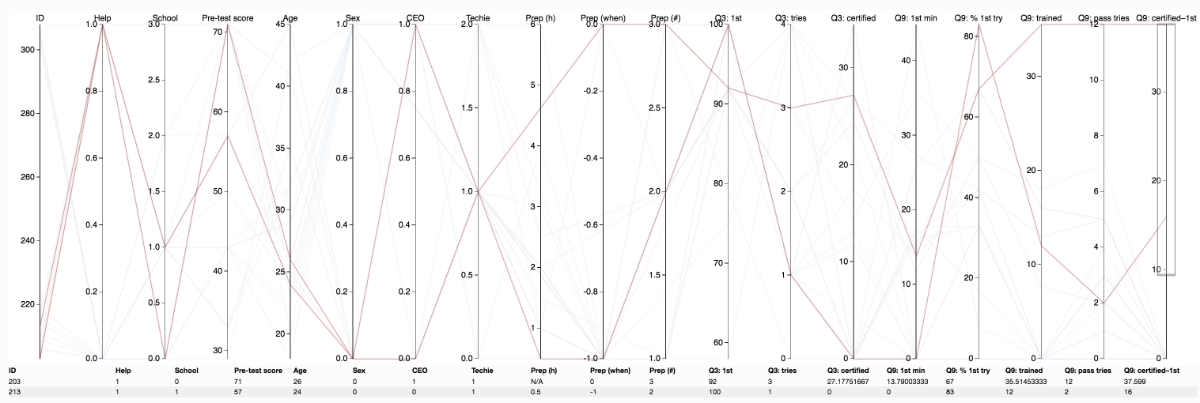
\includegraphics[width=1.0\textwidth]{analysis/paralellCoordinatesWomen.png}
    \caption{The parallell coordinates visualization showing the characteristics of the two coaches that passed the quiz 9 certification.}
    \label{fig:quiz9pl}
\end{figure}

Finally, it is interesting to observe the differences (and lack thereof) between control group A and B. In A, the paper manuals could be read before improving on the quiz results (not during the actual test) The B group were only allowed to observe the right answers within the app, from the score board. In quiz 3, where almost all coaches had 92\% or 100\% immediately, there is no difference observable. However, in quiz 9, the hardest quiz, 5/7 that passed the training were in control group A, and 2/2 that passed the certification were in control group A. An explanation could be that the large amount of questions made the correct answers hard to memorize versus actually learning, or that the ones with manuals felt more supported or motivated because of the extra support.

While these findings could be true for a larger sample, further research needs to be done. The same methods of data analysis are increasingly relevant with a larger data set, and there seems to be correlations and tendencies which are very valuable to look further into.
